\documentclass[journal=jpcbfk]{achemso}

\usepackage[version=3]{mhchem}
\usepackage[T1]{fontenc}
\newcommand*\mycommand[1]{\texttt{\emph{#1}}}
\newcommand{\todo}[1]{\textcolor{red}{#1}}

\usepackage{upgreek}				
\usepackage{xcolor}
\usepackage{booktabs}
\usepackage{multirow}
\usepackage{lmodern}
\usepackage{microtype}

\author{O. H. Samuli Ollila}
\email{samuli.ollila@helsinki.fi}
%\homepage[]{Your web page}
%\thanks{}
\affiliation{Insititute of Biotechnology, University of Helsinki}
\alsoaffiliation{Institute of Organic Chemistry and Biochemistry,
Czech Academy of Sciences, 
Prague 6, Czech Republic}

\author{Harri Heikkinen}
%\homepage[]{Your web page}
%\thanks{}
\affiliation{Insititute of Biotechnology, University of Helsinki}

\author{Hideo Iwa\"i}
%\homepage[]{Your web page}
%\thanks{}
\affiliation{Insititute of Biotechnology, University of Helsinki}



\SectionNumbersOn

\renewcommand{\thetable}{S\arabic{table}}%
\renewcommand{\thefigure}{S\arabic{figure}}%
\renewcommand{\thesection}{S\arabic{section}}%
\renewcommand{\thepage}{S\arabic{page}}%

\title{Supporting Information:\\Rotational dynamics of proteins from spin relaxation times and molecular dynamics simulations}

\begin{document}

\newpage
%\tableofcontents

\section{Supplementary Figures}
\begin{figure*}[!h]
  \includegraphics[width=16.5cm]{../Figs/RMASDplotPsTonBtip4pT310K.eps}%
  \caption{Mean square angle deviations of inertia tensor axes calculated from {\it Pa}TonB-96
simulation with tip4p water model at 310K. The data shown with linear (left) and logarithmic scale
(right).  \label{RMASDplotLOG310}}%
\end{figure*}
\begin{figure*}[!h]
  \includegraphics[width=16.5cm]{../Figs/RMASDplotPsTonBtip4pT298K.eps}%                                                                                                    
  \caption{Mean square angle deviations of inertia tensor axes calculated from {\it Pa}TonB-96
simulation with tip4p water model at 298K. The data shown with linear (left) and logarithmic scale
(right).  \label{RMASDplotLOG310} \label{RMASDplotLOG298}}%                                                                                                                                                  
\end{figure*}

\newpage

\begin{table}[!h]
  \centering
  \caption{Scaling factors of rotational diffusion for different proteins simulated with different water models.
    The last row shows the ratio of simulated and experimental water self-diffusion constant.  }\label{ROTdiffCOEFFSscaled}
  \begin{tabular}{c c c c c c c}
                                       &    & tip3p &  & tip4p && OPC4  \\
    \hline
    {\it Hp}TonB-92                    &    & 2.9   &  & 1     && -\\
    {\it Pa}TonB-96                    &    &  -    &  & 1.2   && -\\
    Calcium recoverin \cite{timr18}    &    &  3.2  &  & -     && -\\
    CBM-64 \cite{heikkinen18}          &    &  -    &  & -     && 1.3 \\
    65K C-RRM \cite{norppa18}          &    & -     &  & 1     && - \\
    &&&&&& \\
    Water self-diffusion \cite{izadi14} &    & 2.4   & & 1.1   &&  1 \\
  \end{tabular}
\end{table}

\bibliography{refs.bib}

\end{document}
